\section{Design \& Konzept}
\label{sec:design-und-konzept}
In diesem Kapitel ...

\subsection{Grundlegende Designentscheidungen}
Bevor auf Entscheidungen eingegangen wird ...

\subsubsection{Android als Plattform}
Das Framework richtet sich ausschließlich an Entwickler die Applikationen für die Plattform Android entwickeln. Es ist damit nicht kompatibel zu iOS, dem Web oder Serverseitigen Anwendungen. Die Spezialisierung lässt es jedoch zu, besser auf mögliche Eigenheiten der Plattform einzugehen. Ein weiterer Grund für diese Entscheidung stellt die Tatsache dar, dass MVI seinen Anfang in der Entwickelung von Webseiten fand und es sich im Fall Android um einen Nachzügler handelt.

\subsubsection{Framework}
Warum Framwork? Besonderheiten...
\subsection{Übersicht der Komponenten im Klassendiagramm}
\begin{sidewaysfigure}
		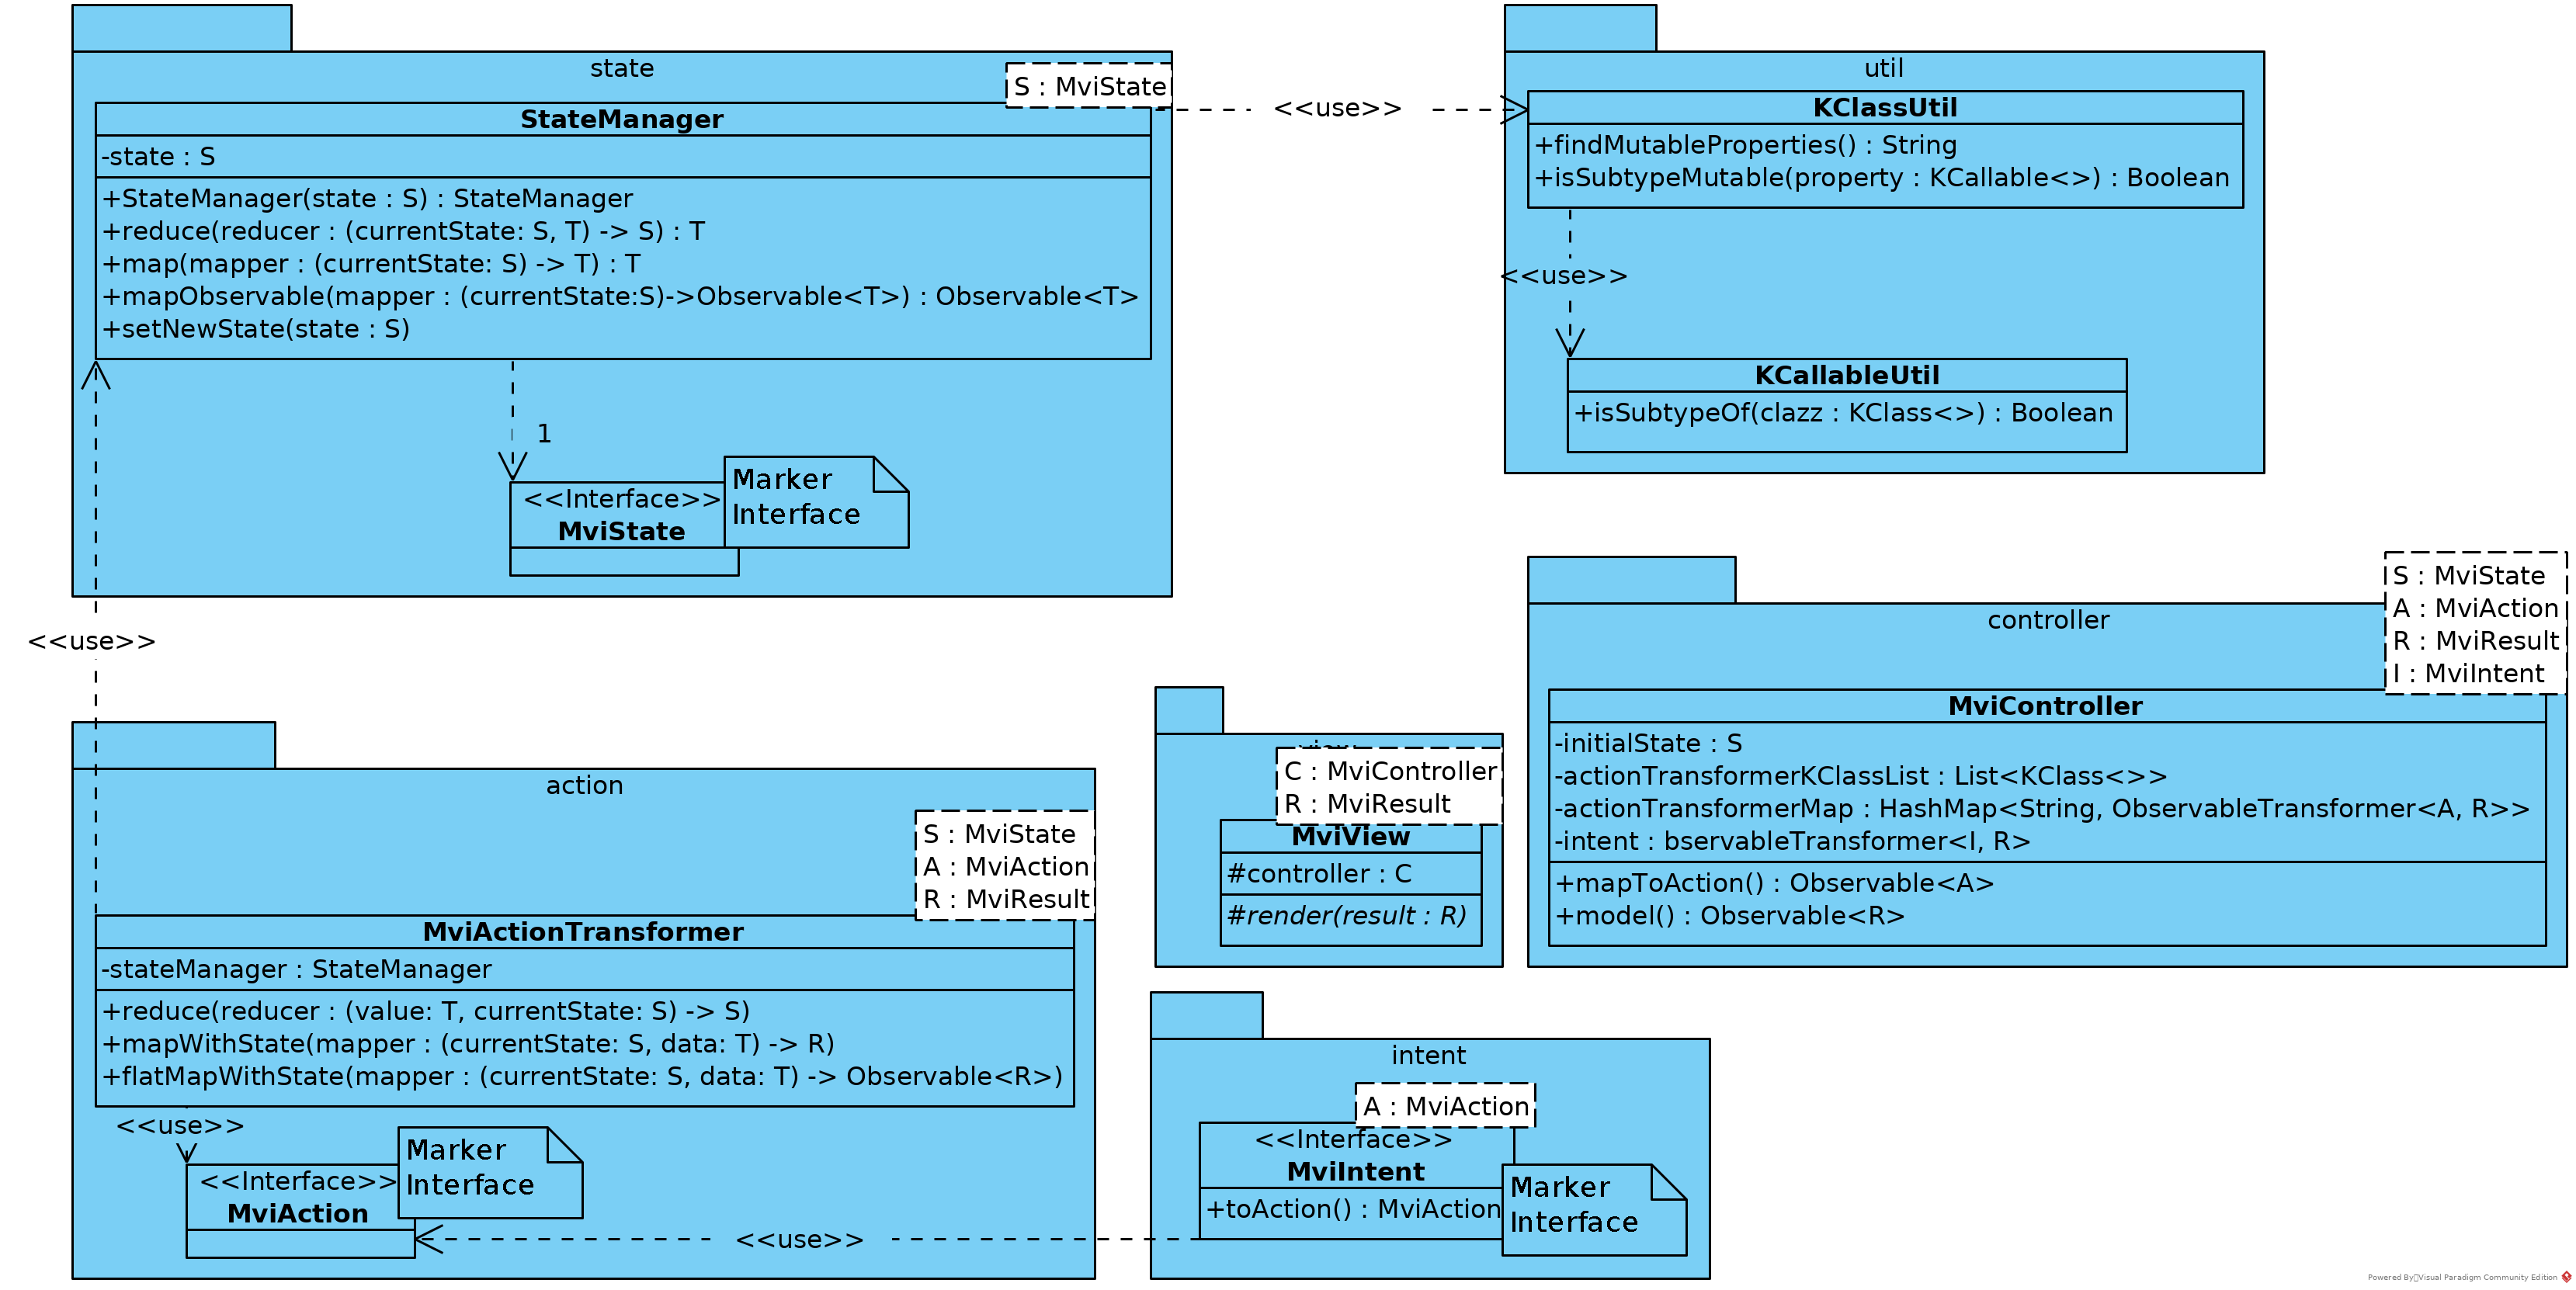
\includegraphics[width=\textwidth]{./images/framework-class-diagram}
		\caption{Komponenten im Klassendiagramm}
\end{sidewaysfigure}
\clearpage
\subsection{Zustand (State) und seine Verwaltung}
In den Ausführungen von MVI wird der Zustand als eine Anhäufung von Werten betrachtet.Es bildet den Kern von MVI und muss im Normalfall vom Entwickler selbst Verwaltet werden. Unter anderem muss garantiert sein, dass ein Zugriff und eine Modifikation des Zustands nur an einer Stelle erfolgen kann. Im Rahmen des Framworks wird eine Komponente genutzt, die diese Aufgaben für den Entwickler übernimmt.
\\
\\
Diese Erwartet den initialen Zustand, der vom Nutzer an das Framework übergeben wird. Innerhalb der Komponente befindet sich Funktionalität, die den Zustand auf seine Korrektheit überprüft. Dazu gehört Beispielweise die Anforderung auf Unveränderlichkeit. Sollte diese nicht gegeben sein, so wird eine Fehlermeldung ausgegeben.
\\
Des weiteren bietet sie Möglichkeiten mit dem Zustand sicher zu arbeiten, sowie eine neuen zu hinterlegen. Diese Komponente ist nicht direkt für den Nutzer zugänglich. Dies verhindert, dass der Zustand an einer beliebigen Stelle verändert werden kann.
\\
\\
Damit das Framework den Zustand besser zuordnen kann, muss es mit einer Beschriftung versehen und dementsprechend markiert werden. Auch diese wird seitens des Framework bereitgestellt.

\subsection{Intent, Action und Result}
Bevor der Entwickler auf den Zustand zugreifen kann, muss er seine Intents definieren. Zu jedem Intent muss eine Action existieren. Hierfür wartet das Framework mit einer Struktur auf, die genanntes erzwingt und die Erfüllung dieser Anforderung sicherstellt. 
\\
\\
Ähnlich wie auf einen Intent eine Action erfolgt, zieht eine Action einen Result nach sich. Auch das gibt das Framework durch eine Struktur vor und muss vom Entwickler angewandt werden. Das Result findet seine Anwendung später in der View.
\\
\\
Sämtliche der hier aufgeführten Strukturen sollten mit ihrem Namen die vorgesehene Intention signalisieren. Zusätzlich müssen sie in der Lage sein weitere Nutzdaten (Payload) aufzunehmen, die mit ihnen in Zusammenhang stehen und für den weiteren Verlauft ausschlaggebend sind.

\subsection{Transformer und die Business-Logik}
Die Action teilt dem Framwork mit, welcher Teil der Business Logik ausgeführt werden soll. Mithilfe einer Komponente, dem 'ActionTransformer', wird vorgegeben an welcher Stelle dies stattfindet. Zu jeder Actio gehört solch ein 'Transormer'. Innerhalb dieser Komponente befindet sich der einzige Ort, an welchem eine Interaktion mit dem Zustand möglich ist.
\\
Der Entwickler kann dabei aus zwei Funktionen wählen:
\begin{enumerate}
	\item Der Zustand wird bereitgestellt und ein neuer wird zurück erwartet
	\item Der Zustand wird bereitgestellt und kann für die zu Ausführende Logik herangezogen aber nicht verändert werden 
\end{enumerate}
\bigskip
Somit ist im Quellcode klar ersichtlich, inwieweit eine Abänderung der Zustands gewollt ist und wann dieser lediglich mitsamt seiner Daten für den weiteren Verlauf benötigt wird. Hinzu kommt hier auch die automatische Handhabung von Seiteneffekten und asynchroner Funktionalität. Dies garantiert, dass der Zustand keine unabsichtliche Modifikation erfährt und zu jedem Zeitpunkt nur einer auf ihn zugreifen kann.

\subsection{Controller}
Der Controller vereint die bisher beschriebenen Komponenten und 'kontrolliert' bzw. koordiniert anhand dieser den Aufruf der Business-Logik. Er stellt das Bindeglied zwischen der View, einer 'Action' und dem dazugehörigen 'ActionTransormer' dar und sorgt für den Aufruf von ebendiesem. Dafür muss er über die vom Entwickler angedachte Form des Zustands, Intents, Action und Result informiert werden. Überdies erhält der Controller den initialen Zustand und eine Liste von Namen der zugehörigen 'ActionTransformer' vom Entwickler.
\\\\
In der initialen Phase verifiziert er daraufhin, dass alle 'ActionTransformer' von der hinterlegten 'Action' und dem 'Result' abstammen um späteren Konflikten vorzubeugen. Anschließend wird der 'StateMananger' mit dem überlieferten Zustand instanziiert. Im letzten Schritt erzeugt der Controller alle 'ActionTransformer' die jeweils einen 'StateManager' zugewiesen bekommen.
\\\\
Im Controller befindet sich die Intent-Funktionen, welche die von der View generierten 'Intents' entgegennimmt und verarbeitet. Sie dient als Einstiegspunk in den unidirektional Kreislauf. Ebenfalls findet hier die Model-Funtionen ihren Platz, welche allerdings nicht für den Entwickler sichtbar ist und intern automatisch abgewickelt wird. Sie trägt Sorge für den Aufruf des korrekten 'ActionTransformers'. 

\subsection{View}
Die 'View' stellt den obersten Teil des Frameworks dar und gibt an, 

\subsection{Anleitung zur korrekten Nutzung}
Hier wird (Schritt für Schritt) beschrieben wie der Entwickler zu Verfahren hat, um das Framework zu nutzen.